\tightsection{Attribute-based Predictability}
\label{predictability}

\jc{There is a serious problem of inconsistent use of quality sample and session. Need to clean up as soon as possible.}

The quality of a video session depends on a variety of factors,
including the network and the CDN. While many of these factors are not
under our control, some of them are. In our case, we assume that we
can control the bitrate of the session, as well as the CDN it streams
from. The challenge is that we do not know what quality will a session
exhibit given a particular choice of the parameters we can
control. This means that making any decision to change the CDN or the
bitrate is more or less like ``shooting in the dark''.

To address this problem, we start with the assumption that the session
quality is correlated to different characteristics (attributes)
associated with the session. Example of such attributes are CDN,
bitrate, ISP, IP address, device, connectivity type, etc. We say that
a session is {\it predictable} if given the values of the attributes
associated with the session we can predict its quality. 

In this section, we formally define {\it predictability}, as well as
provide an upper bound to help us evaluate different prediction
algorithms (\Section~\ref{subsec:upperbound}). We then use our data
set to quantify this upper bound
(\Section~\ref{subsec:videoupperbound}).

%The quality outcome of a session which we would like to predict (which we will call the {\it session under prediction}) intuitively result from a diverse set of factors -- user behavior, network behavior, and CDN behavior, to name a few.  Many of these factors are out of our control; in other cases, a factor may be impacted in principle but its dependence on our decisions is unpredictable.  Our hope in approaching this problem is that some of them, and their causal dependence on decisions we can take, are consistently associated with characteristics we observe about sessions.  As shorthand we say that quality is {\it predictable} to extent that the impact of available decisions can be predicted, with low average error, using the available information about attributes of a session.  The first empirical question we must answer is whether quality is predictable in our dataset. 

%In this section, we first introduce the {\it predictability} and its upper bound of a set of sessions against a simple abstract model of prediction algorithm (\Section~\ref{subsec:upperbound}). Note that since the predictability is defined against a class of prediction algorithms that we consider rather than one specific design, its upper bound provides the insight of the intrinsic difficulty in predicting a set of sessions. We also quantify the predictability upper bound of video quality using our dataset (\Section~\ref{subsec:videoupperbound}). 



\tightsubsection{Definition and model}
\label{subsec:upperbound}

With start with defining the {\it prediction error}.  Given a session
(which we will call the {\it session under prediction}), let $q$ be
the actual quality and $p$ be the predicted quality. Then, the
prediction error $e_{p,q}$ is defined as
\begin{packeditemize}
	\item $e_{p,q}=|p-q|$, in case of buffering ratio and start failure (1 is failure and 0 is success);
	\item $e_{p,q}=|p-q|/q$, in case of average bitrate and join time.
\end{packeditemize}

For a set of sessions under prediction $S=\{s_1,\dots,s_n\}$ let $P=\{p_i\}$ and $Q=\{q_i\}$ be their predicted and actual qualities. respectively ($p_i$ and $q_i$ are the predicted and actual quality of $s_i$). The overall prediction error is then $E_{P,Q}=\left(\frac{1}{n}\sum e_{p_i,q_i}^2\right)^{1/2}$.
\jc{some justification. Henry, i still don't think this is a good way of quantifying error...}

An {\it attribute combination} ({\it AC}) $g$ is a set of attributes. Given an AC $g$, function $v_g$ takes a session $s$ as input and returns an array of values of $s$ on each attribute in $g$. For instance, if $g=[\textrm{ASN, CDN}]$, $v_g(s)=[ASN_s,CDN_s]$ where the client of $s$ belongs to $ASN_s$ and the server belongs to $CDN_s$. An {\it attribute-based prediction algorithm} $P$ \ion{$P$ is also the predicted quality vector, so need to change the notation.} is defined by an AC $g$. $P$ takes a session $s$ as input, and returns $P_g(s)$ as the predicted quality. Note that such an algorithm will provide the same prediction to all sessions with identical attribute values. This means that $P$ cannot provide perfect prediction unless we identify all possible attributes that may impact a sessions's quality, which in practice is infeasible.
 
%To identify the limitation of prediction accuracy when using only the information provided by these attributes, we have the observation that attribute-based prediction algorithm gives the same prediction for all sessions under prediction if their values on every attributes in $g$  is identical. The reason is that any attribute-based prediction algorithm of $g$ does not differentiate two sessions $s_1$ and $s_2$ if $v_g(s_1)=v_g(s_2)$. We call a set of sessions an {\it identical group} of $g$ if they have same value on all attributes in $g$. Then the prediction on any session from an identical group should be the same, i.e., $P_g(s_1)=P_g(s_2)$ if $s_1$ and $s_2$ are from the same identical group of $g$ ($v_g(s_1)=v_g(s_2)$). 

The {\it predictability} of AC $g$ over a set of sessions $S$ is given by the minimal overal prediction error over all prediction algorithms on $g$, i.e., $p^*=\textrm{argmax}E_{P,Q}=\textrm{argmax}_p\left(\frac{1}{n}\sum e_{p,q_i}^2\right)^{1/2}$. For example, in the case of buffering ratio, $p^*$ is the mean of $q_i$. Therefore, the predicability of $g$ over a session set $S$ is the minimal overall prediction error $R_g(S)=E_{P^*,Q}$ where $P^*$ gives the same optimal prediction $p^*$ for each session in $S$. This definition can be extended to any set of sessions $S$ by dividing sessions into identical groups of $g$, and use the optimal prediction for each identical group to be the prediction of sessions in it, i.e., $R_g(S)=E_{P^*,Q}$ where prediction of $s_i$ in $P^*$ is the optimal prediction of the identical group that $s_i$ belongs to.\ion{This is a very confusing paragraph.}

% is a measure of the capacity of all attribute-based prediction algorithms that use $g$ as AC. We first consider an identical group of $g$, $S=s_1,\dots,s_n$, and let their quality be $q_1,\dots,q_n$ and the prediction should be the same value $p$. Then, we will have an optimal prediction $p^*=\textrm{argmax}E_{P,Q}=\textrm{argmax}_p\left(\frac{1}{n}\sum e_{p,q_i}^2\right)^{1/2}$. For example, in the case of buffering ratio, $p^*$ is the mean of $q_i$. Therefore, the predicability of $g$ over a session set $S$ is the minimal overall prediction error $R_g(S)=E_{P^*,Q}$ where $P^*$ gives the same optimal prediction $p^*$ for each session in $S$. This definition can be extended to any set of sessions $S$ by dividing sessions into identical groups of $g$, and use the optimal prediction for each identical group to be the prediction of sessions in it, i.e., $R_g(S)=E_{P^*,Q}$ where prediction of $s_i$ in $P^*$ is the optimal prediction of the identical group that $s_i$ belongs to.

The predictability quantifies the dispersion in quality of the sessions that an AC cannot differentiate. Ideally, if the attributes in AC $g$ selected reflect all the factors that determine the quality of a session, then the sessions in an identical group of $g$ should produce the same quality and the upper bound is exactly one. 

\jc{The current definition predictability is weird as it gives smaller value to more predictable set of sessions. }


\begin{figure*}[t!]
\centering
\subfigure[Predictability of temporal attributes]
{
	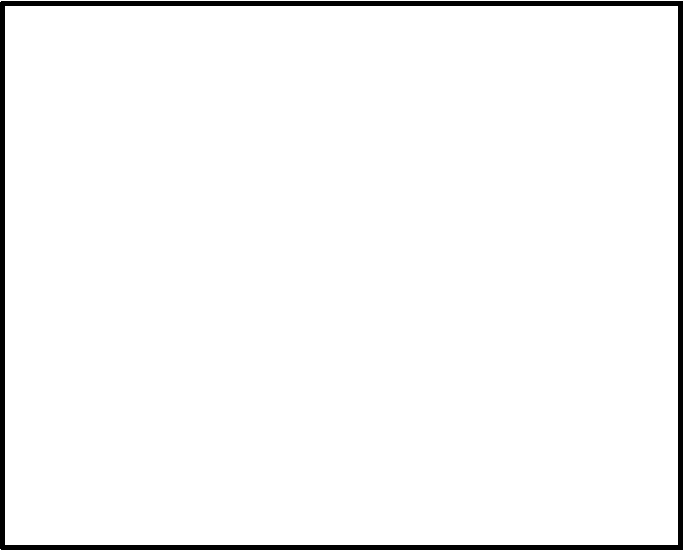
\includegraphics[width=0.2\textwidth]{figures/placeholder.pdf}
	\label{subfig:predictability:temporal}
}
\subfigure[Predictability of spatial attributes]
{
	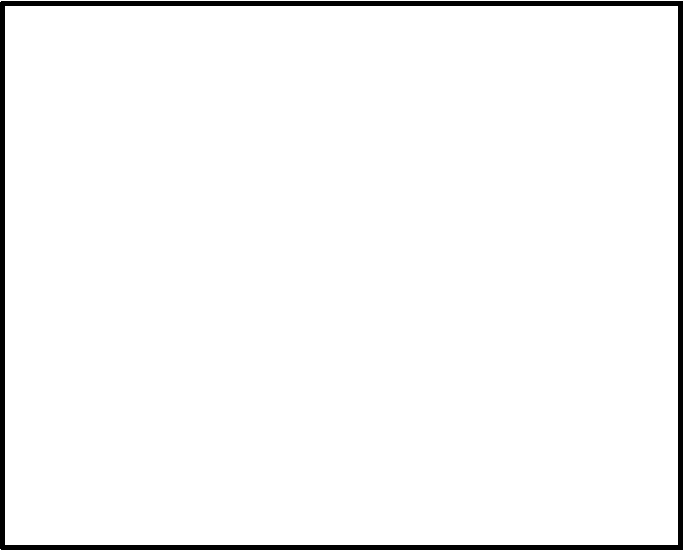
\includegraphics[width=0.2\textwidth]{figures/placeholder.pdf}
	\label{subfig:predictability:temporal}
}
\subfigure[Rank of predictability among ASN]
{
	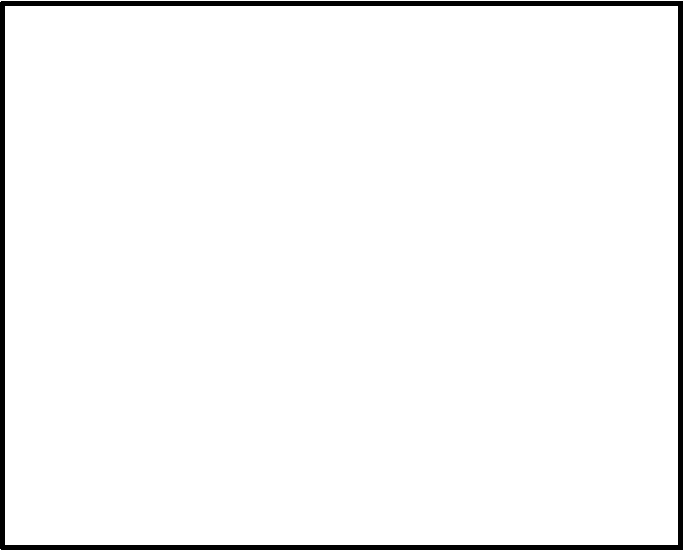
\includegraphics[width=0.2\textwidth]{figures/placeholder.pdf}
	\label{subfig:predictability:asn}
}
\subfigure[Rank of predictability among Site]
{
	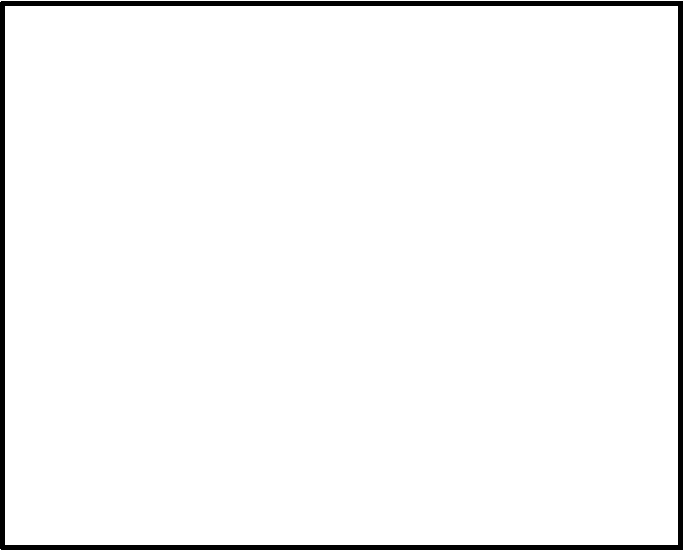
\includegraphics[width=0.2\textwidth]{figures/placeholder.pdf}
	\label{subfig:predictability:site}
}
\tightcaption{Quantifying predictability over our dataset.}
\label{fig:predictability}
\end{figure*}


\tightsubsection{Predictability over video quality samples}

In this section, we quantify the predictability of the session attributes in our dataset. Note that, measuring the predictability assumes an oracle approach as it requries the knowledge of all sessions under prediction. Also note that predictability is not necessarily a tight lower bound of overall prediction error, as it does not guarantee that there exists of a prediction algorithm that can match the minimal overall quality error based on historical data only. Despite these limitations, predictability is a valuable bound to compare prediction algorithms agianst. We consider the set of spatial attributes introduced in \Section~\ref{subsec:dataset} as well as a set of time intervals as temporal attributes.

%spatal attributes. In addition, we use different temporal interval as temporal attributes. Given the same spatial attributes, temporal attributes (e.g., 1 minute) indicate the granularity in time which we use to differentiate sessions. Given the same temporal attributes, the spatial attributes (e.g., ASN, CDN) indicate the aspects of a session that we believe can make an impact on the quality.

\myparatight{Temporal attributes} Figure~\ref{subfig:predictability:temporal} shows the predictability of different temporal attributes (time granular) combined with all spatial attributes. An example of an AC with a $5$-minute temporal attribute is [5-minute, ASN, Object, Site, Initial CDN, Initial Bitrate, OS, ConnectionType]. Each point in the figure represents the overall predictability for a given time period. The predictability tends to be better for small intervals. As the interval length increases the predictability stabilizes.
%The figure shows that with different granulars do have impact on predictability. Smaller intervals are more predictable, but the predictability becomes similar after granular is less than about 5 minutes.

\myparatight{Spatial attributes} Figure~\ref{subfig:predictability:temporal} shows the predictability of different spatial attributes combined with the $5$ minute temporal attribute. Again, the finest spatial attribute combination is [ASN, Object, Site, Initial CDN, Initial Bitrate, OS and ConnectionType].  Instead of showing all ACs with these attributes (in total $2^7-1=127$ ACs), we group them by their number of attributes and show the ones with best predictability. This illustrates the impact of the number of attributes on predictability. The results show clear improvements as we use more attributes, though we reach diminishing return when we approach seven attributes.

\myparatight{Different partitions} The above results show that predictability varies significantly with the attributes we consider. Next, we present the predictability also varies across different partitions of the same AC (e.g., ASN, Site). Figure~\ref{subfig:predictability:asn} (/\ref{subfig:predictability:site}) shows the distribution of the mean predictability among top-$k$ and last-$k$ ASNs (/Sites). These results confirm that predictability vary significantly across different partitions. 
%More importantly, this suggests that for some classes of clients, the video quality is more predictable than for other classes of clients by using the attributes we collect.

\comment{
\tightsubsection{Summary of observations}
\begin{packedenumerate}
	\item The overall prediction accuracy
\end{packedenumerate}
}

\tightsection{Challenges of Prediction Algorithms}

\comment{
We then investigate a naive prediction algorithm that make prediction by only looking at sessions sharing exact values on all attributes, and categorize its reasons and limitations. 

%In this section, we provide some rough statistics that indicate that quality is somewhat predictable, and then raise some challenges that must be solved by a practical algorithm for prediction.


\tightsubsection{Quality similarity between close sessions}
We observe {\it spatial} and {\it temporal} attributes of each session.  These attributes can be used to define a distance between sessions.  Intuitively, sessions that match exactly on all observable attributes are most likely to be similar.  If we have a large number of sessions exactly matching the session whose quality we would like to predict (which we will call the {\it session under prediction}), the obvious algorithm to predict quality outcomes given a particular decision simply returns the actual distribution (i.e. the CDF) of quality outcomes for those matching sessions for which that decision was taken.  Since we would like to compare decisions quickly, it is useful to summarize a prediction in a single number like the mean of this distribution; this is the approach we take.  Thus in the presence of infinite data we would take as our prediction the mean quality outcome of sessions exactly matching the session under prediction.  For reasons we will discuss shortly, we may want to relax the requirement of exact matching to mere closeness.  Along {\it spatial} dimensions, two sessions are close if they share same value on one or multiple attributes. For example, two sessions could be from the same ASN, or using the same CDN or from the same ASN to the same CDN. The spatial attributes we observe are mostly categorical, so the only useful distinction with respect to a single attribute is between a match and a non-match. Two sessions are temporally close if they occur at roughly the same time.

To motivate that quality is predictable using the available attributes, we start with examining similarity of quality samples if spatially, they share the value on all attributes and temporally, they come from the smallest possible time window (i.e., one minute).
Happily, quality samples that are spatially and temporally close typically have similar quality; so quality is somewhat predictable using the available attributes.

\begin{figure}[h!]
\centering
 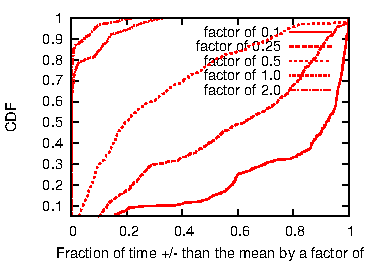
\includegraphics[width=0.4\textwidth] {figures/spatial-similarity.pdf}
\tightcaption{Spatial similarity of quality (average bitrate) among the sample of [Site, Initial CDN, Initial Bitrate, ASN, Site, ConnectionType, Object]. Each point represents a group of quality samples}
\label{fig:spatial-similarity}
\end{figure}

\myparasum{Spatial similarity} Spatial similarity is between the quality samples collected at the same time interval from sessions that share certain attribute values. \jc{Figure: x-Fraction of time less/greater than mean by various factor, y: CDF} Figure~\ref{fig:spatial-similarity} quantifies the similarity of average bitrate in quality samples that share the same tuple of Site, Initial CDN, Initial Bitrate, ASN, Site, ConnectionType, Object. It shows that there is a large fraction (more than 50\%) of quality sample groups that have less than 20\% of quality sample less or greater than the mean of this group with a factor of 0.5.

\begin{figure}[h!]
\centering
 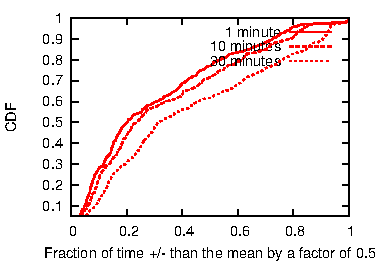
\includegraphics[width=0.4\textwidth] {figures/temporal-similarity.pdf}
\tightcaption{Quantifying impact of temporal distance on quality similarity. Figure shows likelihood of being more than a factor of 0.5 away from mean quality for all [Site, Initial CDN, Initial Bitrate, ASN, Site, ConnectionType, Object] groups with increasing (from left to right) time scales.}
\label{fig:temporal-similarity}
\end{figure}

\myparasum{Temporal similarity} Temporal similarity is between the average quality collected in different time interval of the same group of sessions that share certain attribute values. In Figure~\ref{fig:temporal-similarity}, we compare the similarity between quality samples with certain distance in time, and quantify the impact of temporal distance on quality similarity. Each point represents a group with the fraction of quality samples that is less or greater than the mean of the quality samples that have the same values on all seven attributes $t$ minutes ago ($t=1,10,30$). It shows that temporal distance does impact the quality similarity. 

\comment{
\myparasum{Summary of key observations} \jc{mostly based on my previous experience. subject to change after formal results are generated.}
\begin{packedenumerate}
	\item Both similarity of quality samples show that it is feasible to predict the quality of a new session and its decision by looking at quality samples that are spatially and temporally close to it.
	\item Spatial similarity varies across different attributes.  Using more attributes can improve things.
	\item Different quality metrics have different level of similarity, especially, buffering ratio has the largest similarity.
\end{packedenumerate}
}
}









Having shown that with the attributes we collect, it is possible to achieve good predictability (i.e., low overall prediction error), we now present the challenges in designing a prediction algorithm that can reach such prediction error in practice. In particular, a practical algorithm can only use the information (quality samples) collected before the minute that the session under prediction belongs to.

First, we categorize the sources of difficulty in predicting video quality accurately (\Section~\ref{subsec:challenges}) which inform the choice of aggregating identical groups of all attributes (i.e., the finest identical groups) by ignoring (hopefully, less important) attributes so that more samples will be used(\Section~\ref{subsec:aggregation}) to counteract the noise and estimation error brought by sparse data.

\tightsubsection{Predicting from finite data}

\label{subsec:challenges}
Although the figures~\ref{fig:predictability} show that in many cases, quality is similar among quality samples that share the same attribute values and same temporal interval, there are still a lot of quality sample groups that have high dispersion. This is one of the key challenges that make quality prediction difficult. 
In this part, we enumerate the potential reasons that causes the dispersion we observe. Intuitively, if the number of similar sessions is small (e.g., $~10$ sessions), the mean quality outcome is subject to considerable random noise.  If we use this mean for prediction, the prediction will be subject to the same noise and consequently to high average error.  As the number of attributes grows, quality grows more predictable (as the noise decreases) but the number of perfectly-matched sessions may drop exponentially.

Of course, prediction in the presence of limited information is statistics problem, and there are many potential solutions to this problem.  In general, there are four sources of prediction error:
%Any solution will deal with, and potentially trade off, four sources of prediction error:

\begin{packedenumerate}
  \item \emph{Estimation error:} In the statistical literature, prediction error due to limited data is often called {\it estimation error}.  Even other things being equal, more data produce more accurate prediction. For example, Figure~\ref{fig:group-size-impact} presents the prediction error vs. group size (i.e., number of samples). Given a large number of attributes, estimation error is a serious problem in practical.  Using all available attributes, many sessions have very few matches, as we would expect given the exponential explosion in combinations of attribute values.  

\begin{figure}[h!]
\centering
\subfigure[Prediction error vs. group size (w.r.t average bitrate)]
{
        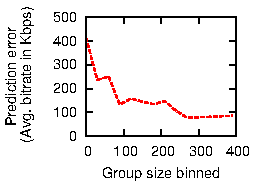
\includegraphics[width=110pt]{figures/count-err.pdf}
	\label{subfig:group-size-impact:count-err}
}
\subfigure[Distribution of group size]
{
        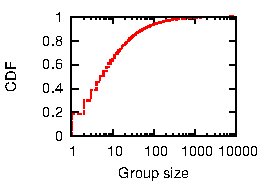
\includegraphics[width=110pt]{figures/count-cdf.pdf}
}
\tightcaption{Impact of group size (i.e., number of samples in a group). They show that more samples give more accuracy, but most of groups do not have sufficient samples for accurate prediction.}
\label{fig:group-size-impact}
\end{figure}

  %\item \emph{Bias} due to missing or unused information: When grouping quality samples according to attributes we observe, we of course may not observe attributes that are important for prediction.  Say we do not observe (or use) important attribute X.  Then, even if we have infinitely many sessions that match the current session on all observed attributes, the average outcome for all of those sessions may be different from the average outcome for the subset of sessions that match the current session on attribute X.  This is a form of bias.  Predictability, as we have defined it, simply means low bias.  Importantly, it is not alleviated by gathering more session data; as we have seen, it may be alleviated by gathering more attributes about each session.
\item \emph{Bias} due to missing or unused information: The bias occurs when we do not observe (or use) an attribute, $X$, that is important for prediction. Then, even if we have infinitely many sessions that match the current session on all observed attributes, the average outcome for all of those sessions may be different from the average outcome for the subset of sessions that match the current session on attribute $X$.  Thus, the bias is not alleviated by gathering more session data, but by gathering more attributes about each session.
  %\item \emph{Unavailability of recent data:} In a practical system, there are delays in measuring, sending and processing quality samples, so they are not available instantly.  If conditions change rapidly, there may be no quality samples sufficiently close to the session under prediction.  This is an extreme example of estimation error.  In this case it may be necessary to model the evolution of the video ecosystem over time in order to extrapolate to the current time. Figure~\ref{fig:quality-variability} shows per-minute quality variability. It shows that even with sufficient data, the mean value of a group of quality samples could vary significantly.
\item \emph{Unavailability of recent data:} In a practical system, there are delays in measuring, sending and processing quality samples, so they are not available instantly.  If conditions change rapidly, there may be no quality samples sufficiently close to the session under prediction.  This is an extSreme example of estimation error.  In this case it may be necessary to model the evolution of the video ecosystem over time in order to extrapolate to the current time. Figure~\ref{quality-variability} shows per-minute quality variability. It shows that even with sufficient data, the mean value of a group of quality samples could vary significantly.

\begin{figure}[h!]
\centering
 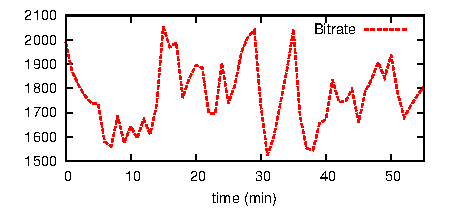
\includegraphics[width=0.4\textwidth] {figures/quality-time.pdf}
\tightcaption{Temporal variability of quality. The figure shows the mean value of average bitrate of a fixed group of same [Site, Initial CDN, Initial Bitrate, ConnectionType, ASN, Object], which has 100 quality samples in every minute in the figure.}
\label{fig:quality-variability}
\end{figure}

  \item \emph{Noise:} Even if we observed all conceivable attributes of a session and had infinitely many examples of exactly quality samples, outcomes may be affected by non-deterministic inputs.  For example, performance may be affected by exponentially backoff at the data link layer or the congestion generated by cross traffic at the network layer. This implies that some degree of prediction error is inevitable.
\end{packedenumerate}

Next, we formalize the prediction error (see \cite{domingos2000unified} for a less specialized discussion of the decomposition of prediction error).  Let $D$ be a set of quality samples from which a prediction algorithm learns its predictions.  Let $p_i$ be the predicted quality for session $i$ and $q_i$ be its actual quality.  We further assume that $q_i$ is fixed except for an independent additive noise component, i.e. $q_i = \hat{q}_i + \epsilon_i$, where $\hat{q}_i$ is non-random and $\epsilon_i$ is a random variable with mean $0$, independent of $p_i$.  Then the mean squared prediction error of $p_i$ is:

\begin{align}
  \label{eqn:biasvariance}
  \E_D[(p_i - q_i)^2] &= \Var_D[p_i - q_i] + (\E_D[p_i - q_i])^2
\end{align}
\begin{align*}
  \label{eqn:biasvariancelong}
  &= \Var_D[p_i - \hat{q}_i - \epsilon_i] + (\E_D[p_i - \hat{q}_i - \epsilon_i])^2 \\
  &= \Var_D[p_i - \hat{q}_i] + \Var_D[\epsilon_i] + (\E_D[p_i - \hat{q}_i - \epsilon_i])^2\\
  &= \Var_D[p_i] + \Var_D[\epsilon_i] + (\E_D[p_i - \hat{q}_i - \epsilon_i])^2\\
  &= \Var_D[p_i] + \Var_D[\epsilon_i] + (\E_D[p_i - \hat{q}_i] - \E_D[\epsilon_i])^2\\
  &= \Var_D[p_i] + \Var_D[\epsilon_i] + (\E_D[p_i] - \hat{q})^2
\end{align*}

The first term in equation \eqref{eqn:biasvariancelong} is estimation error -- the variability in predictions across possible sets of observed data.  It will increase as the number of sessions similar to session $i$ in $D$ decreases. As a special case, it may be very large if only a few quality samples in $D$ are temporally close to session $i$.  The second term is noise.  The third term is the squared bias of the predictor, which does not generally decrease with the size of $D$.  The average prediction error is simply the average over all these three terms of sessions $i$. 

\tightsubsection{Aggregation}
\label{subsec:aggregation}
A simple strategy to reduce estimation error is {\it aggregation}~\cite{any citation?}.  By aggregation we mean putting quality samples into coarser groups that match on only a subset of observed attributes.  Aggregation increases the number of samples in each identical group by reducing the number of attributes, thus reducing estimation error at the cost of increased bias. 
Intuitively, when estimation error is small (say, when a fine-grained identical group contains many sessions) we want to eliminate bias by using a fine-grained group.  When estimation error is large, we want to aggregate more.  \comment{Figure \fillme demonstrates this for \fillme\jc{nice to have a figure to confirm such tradeoff does happen in our dataset.}.}  This indicates that a prediction algorithm that uses aggregation should pay attention to its error rate to determine the right degree of aggregation.


\begin{figure}[h!]
\centering
 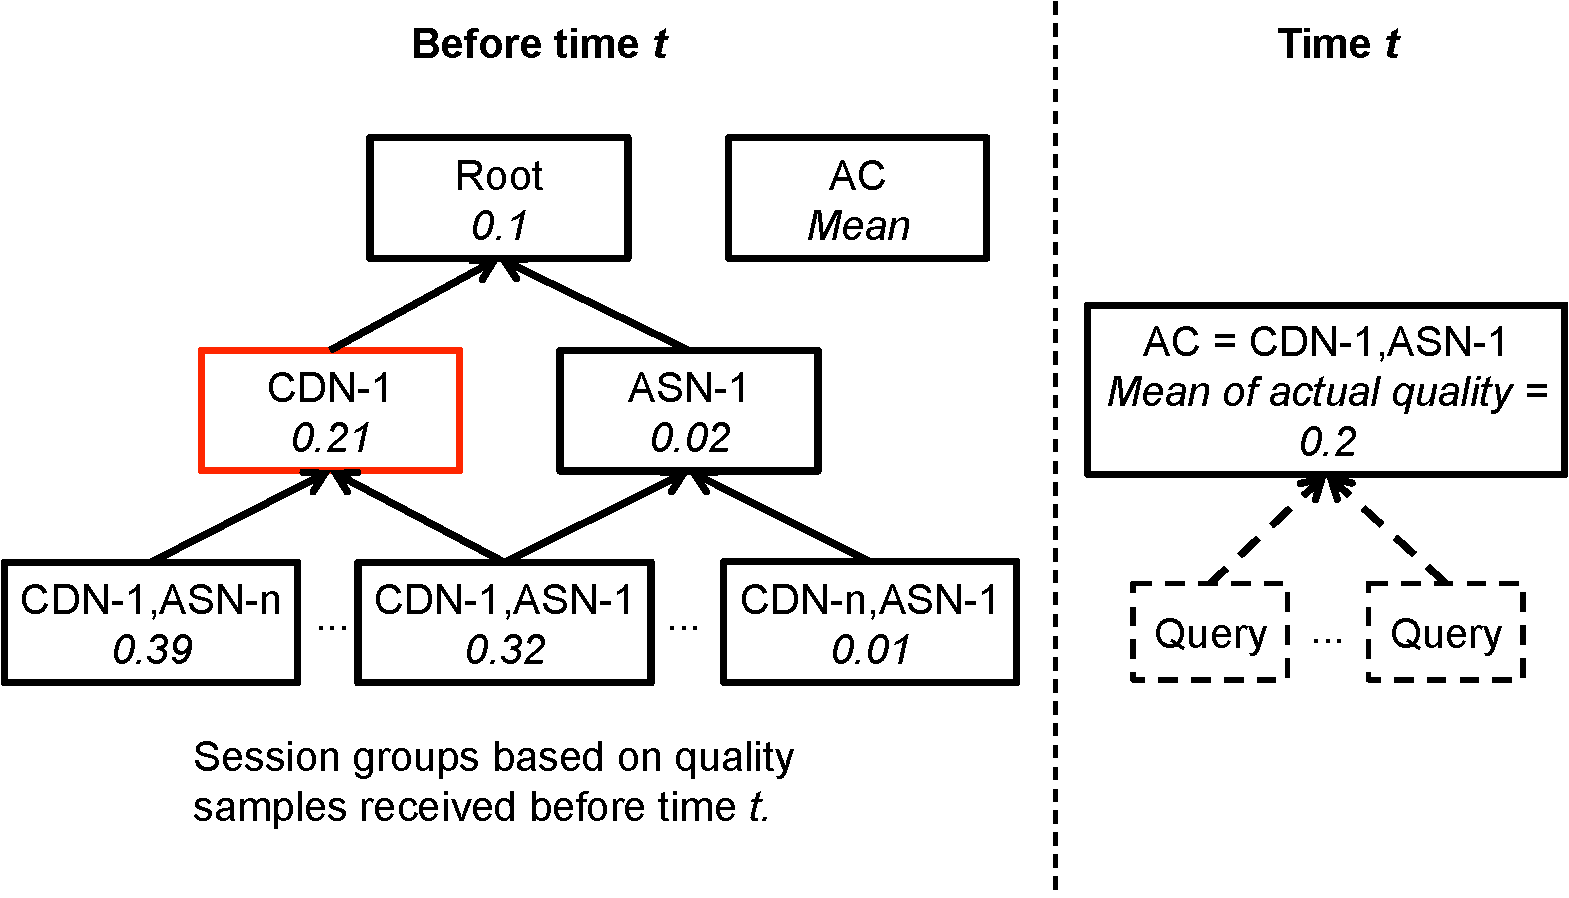
\includegraphics[width=0.5\textwidth] {figures/fig-optimal-AC.pdf}
\tightcaption{Example of how optimal AC is identified. The optimal AC is colored in red. Assuming the considered attributes are fixed, the optimal AC assumes that all sessions that belong to the same finest group should be given the same prediction, and the optimal AC is the one that gives the closest prediction among those that contain this finest group.}
\label{fig:example-optimal-ac}
\end{figure}

We use a simple methodology, called {\it optimal AC}, to show the dynamics of the right degree aggregation. For a finest identical group at $t$-th minute, we first build a hierarchy that consists of all degrees of aggregation over the quality samples we collects before the $t$-th minute. Figure~\ref{fig:example-optimal-ac} shows an example of three attributes. 
Then, the optimal AC for this identical group is the degree of aggregation that gives the prediction value closest to the optimal prediction for the finest identical group at $t$-th minute which yields to minimal prediction error.
For instance, if the optimal prediction of the targeted identical group is 0.2, the optimal AC (colored in red) is the one with the closest prediction to 0.2, i.e., $(ASN, CDN)$. 


\begin{figure}[h!]
\centering
\subfigure[Distribution of coverage of top five optimal ACs (w.r.t averge bitrate).]
{
        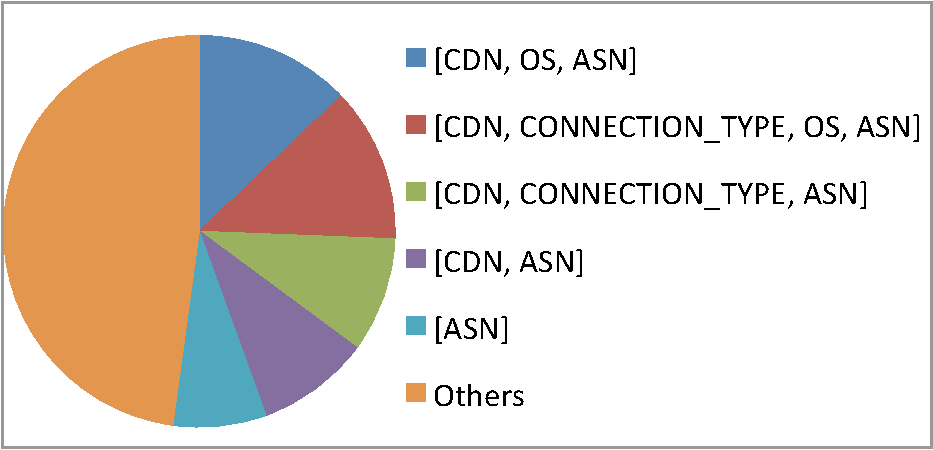
\includegraphics[width=0.4\textwidth]{figures/optimal_AC_distribution.pdf}
}
\subfigure[Prevalence of pair of (session under prediction, optimal AC).]
{
        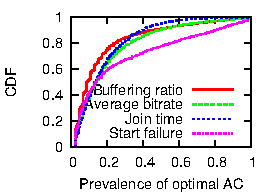
\includegraphics[width=0.33\textwidth]{figures/optimal-prevalence.pdf}
}
\subfigure[Persistence of pair of (session under prediction, optimal AC).]
{
        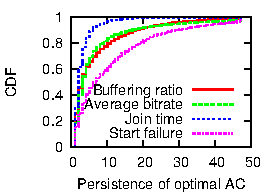
\includegraphics[width=0.33\textwidth]{figures/optimal-persistence.pdf}
}
\tightcaption{Dynamics of the optimal AC. (a) gives coverage of optimal ACs (for each AC, the fraction of sessions of which this AC is the optimal AC).
(b) gives prevalence of pair of (session under prediction, optimal AC) (the fraction of time that the finest group has this optimal AC).
(c) gives persistence of pair of (session under prediction, optimal AC) (i.e., the longest continuous duration where a finest group has the same optimal AC).}
\label{fig:optimal-ac-dynamics}
\end{figure}

\myparatight{Optimal AC} We find that the optimal AC (the aggregation that gives minimal prediction error) is in many cases neither the finest nor the coarsest one, and, in addition, is highly dynamic:
 
\begin{packeditemize}
	\item {\it No single optimal AC:} Figure~\ref{fig:optimal-ac-dynamics}-(a) shows the coverage of optimal ACs, i.e., the fraction of time for which a given AC is the optimal AC. Note that there is no single optimal AC. For example, the finest group only has coverage about 20\% and no coarsest grain AC (single attribute) is among the top 5. This implies that the optimal AC is often in between.
	\item {\it No temporally prevalent optimal AC:} Figure~\ref{fig:optimal-ac-dynamics}-(b) shows the prevalence of the $($\emph{session-under-prediction, optimal AC}$)$ pairs, i.e., the fraction of time the fines group of sessions has the same optimal AC. Note that $70\%$ pairs only last for less than $20\%$ of time. This implies that there is no single or a small set of optimal ACs that can cover most sessions.
	\item {\it Highly dynamic optimal ACs:} Figure~\ref{fig:optimal-ac-dynamics}-(c) shows the persistence of the $($\emph{session-under-prediction, optimal AC}$)$ pairs, i.e., the longest continuous duration where the finest group has the same optimal AC. Only 40\% of pairs last for more than 10 minutes. This suggests that even with a reactive strategy will be challenging to track the optimal ACs.
\end{packeditemize}



